\documentclass[a4paper,12pt,titlepage]{scrartcl}
\usepackage{graphicx}

\titlehead{
	\centering
	
\includegraphics[width=5in]{images/d3b.png}
	
\includegraphics[width=5in]{images/kidsfirst.png}
}
\title{Developer Handbook}
\date{\today}

\begin{document}

	\maketitle
	
	\tableofcontents
	\newpage
   
	\section{Welcome}
   
	\section{Creating Issues}
	
	Issues should be created 
	If a repository has an {\em Issue Template}, make sure to follow it!
      
	\section{Finding Issues}
	
	\subsection{Labels}
	
	Repositories across the D3b Github organization that have frequent user feedback and bug reports should use our standard set of labels to tag issues shown in Figure \ref{fig:labels}.
	Labels act as a means of filtering categories of issues and providing summaries of effort completed in release notes.
	Users that are not part of the organization may not add labels themselves, so please add labels as you see necessary to new issues.
	The {\b help wanted} label is a special label that is displayed in repository summaries on Github (See the {\em 11 Issues need help} in Figure \ref{fig:reposummary}).
	Use it to mark issues that are self-contained and do not require in-depth knowledge of how the code base works.
	This tag is useful for guiding new members or external contributors looking to get involved to issues that will be easy for them to accomplish.
   
    \begin{figure}
    		\centering
    		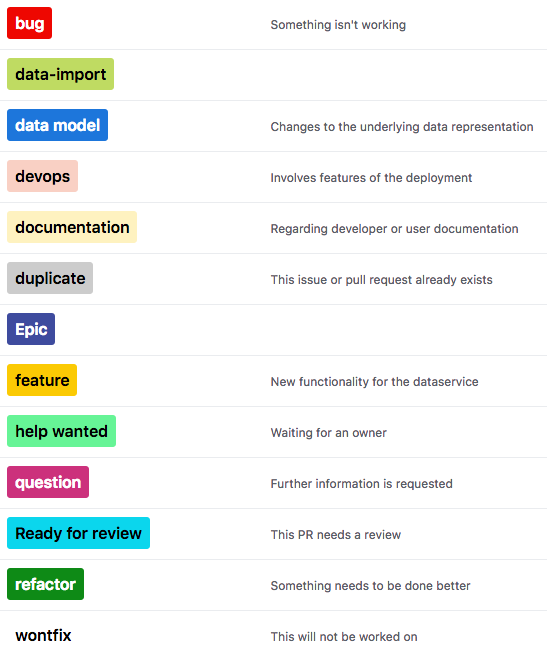
\includegraphics[width=0.6\linewidth]{images/labels.png}
    		\label{fig:labels}
    		\caption{Standard Repository labels with descriptions and colors}
    \end{figure}
	
   
	\section{Creating a Pull Request}
	
	\subsection{Commit Messages}
	
	\subsection{Pull Request Titles}
	
	\subsection{Keeping the Commit Log Tidy}
	
	\subsection{Labeling Pull Requests}
	
	\subsection{Requesting Reviews}
   
	\section{Review Process}
	
	\subsection{Code Review}
	
	\subsection{Testing}
	
	\subsection{Status Checks}
   
	\section{Software Release}
	
	\section{New Repositories}
	
	\begin{figure}
    		\centering
    		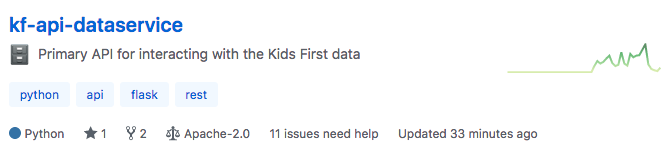
\includegraphics[width=0.6\linewidth]{images/reposummary.png}
    		\label{fig:reposummary}
    		\caption{An exemplary repository summary including: proper naming scheme, emoji followed by short description, labels, the {\em Apache 2.0} license, and issues tagged with {\em help wanted}}
    \end{figure}
   
\end{document}